\subsection{Messverfahren}
\paragraph{Aufgabe 1:} Vorversuch: Es wird einfach qualitativ die Spannungsänderung der Induktionsspule beobachtet, wenn ein
Stabmagnet in der Spule bewegt wird bzw. die Spule bewegt wird. Hier ist die wichtige Beobachtung, dass nur die Relativbewegung beider Geräte relevant ist. 

\paragraph{Aufgabe 2:} Zunächst wird die Helmholtzspule an Gleichstrom angeschlossen und ein Motor betreibt die Induktionsspule über einen Gummiriemen an. Die gemessene, induzierte Spannung an der Flachspule (= Induktionsspule) wird am Oszilloskop aufgezeichnet. Es wird eine Messreihe aufgenommen, bei der unter konstantem Gleichstrom die Motorfrequenz erhöht und einmal unter konstanter Frequenz der Strom erhöht wird. Es wird jeweils die Amplitude oder der Effektivwert der Wechselspannung am Oszilloskop abgelesen.

\paragraph{Aufgabe 3:}  Die von einem Sinusgenerator erzeugte Wechselspannung, mit der die Helmholtzspule betrieben wird, kann am genauso wie die Induktionsspannung am Oszilloskop angezeigt werden. Die Flachspule wird zunächst auf \(\ang{0}\) gedreht und für die erste Messreihe die Amplitude der induzierten Spannung bei verschiedenen Winkeln der Flachspule gemessen. Für eine zweite Messreihe wird die Frequenz der Eingangsspannung stufenweise erhöht und die Spannung \(U_H\), die über die Helmholtzspule abfällt, der fließende Strom \(I_H\), sowie die Amplitude der induzierten Spannung gemessen werden. 

\paragraph{Aufgabe 4:} In Aufgabe 4 wird das Magnetfeld in der Helmholtzspule so erzeugt, dass es die vertikale Erdmagnetfeldkomponente ausgleicht. Dazu wird bei konstant drehender Induktionsspule die Stärke des Spulenmagnetfelds durch Verstellen des Stroms variiert, bis die gesamte Induktionspannung ein Minimum aufweist, in diesem Fall kompensiert die Helmholtzspule die ganze Vertikalkomponente und nur die Horizontalkomponente des Erdmagnetfelds trägt zur Induktion bei. 
\vfill
\subsection{Messprotokoll}
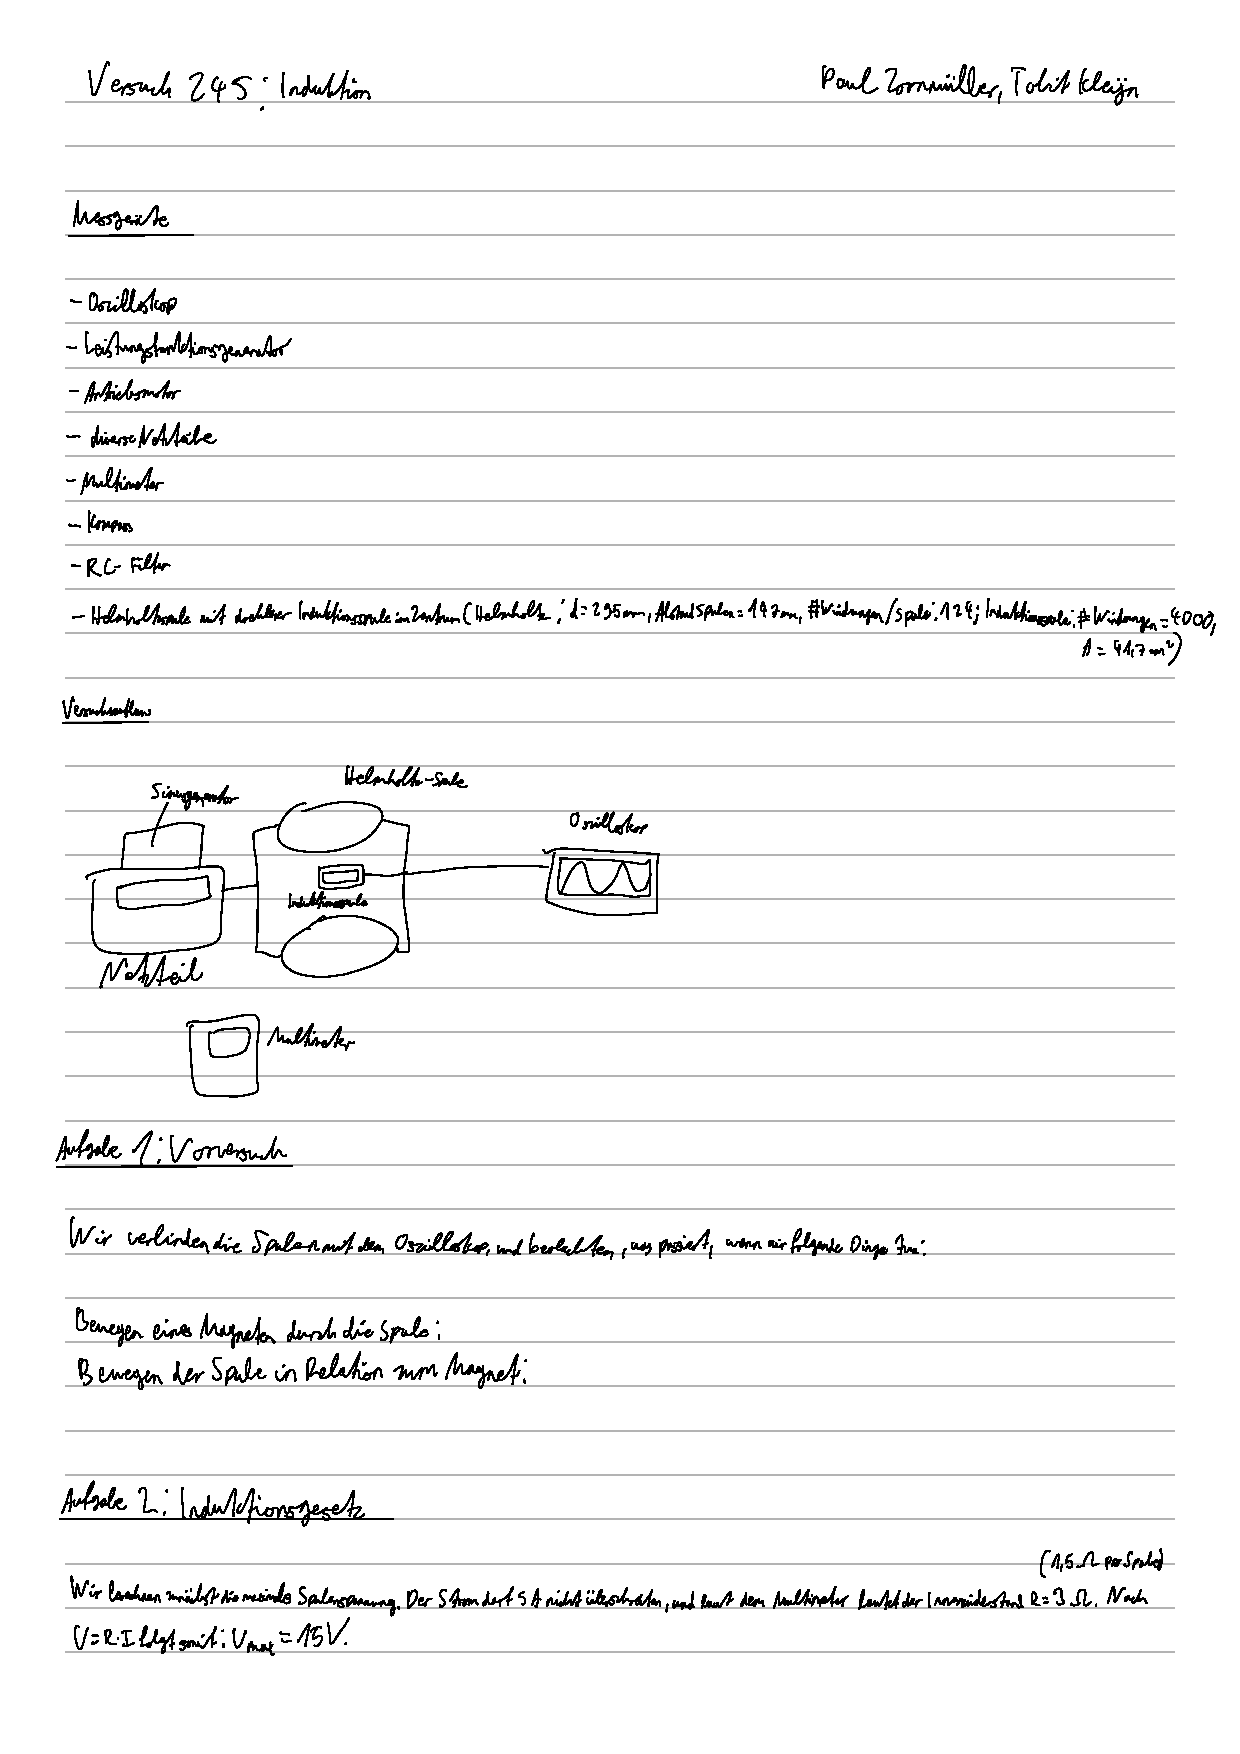
\includepdf[pages=-]{./images/245.pdf}
% heibox.uni-heidelberg.de/d/a48f9d7b91264990a16e/
